\chapter{Parallelization}\label{sec:mpi}

\section{Domain decomposition}

The domain decomposition is performed along the first and last indexes,
typically $i$ and $k$, respectively, that is, along directions $Ox$ and
$Oz$. Initially, the code only supported 1D decomposition along $Oz$, the
outer-most index. The reason to chose that direction was to simplify I/O and to
maintain homogeneity in the serial part of the algorithm (the largest part) for
the cases with periodicity along that direction (boundary conditions where only
needed in the other two directions, for instance, in a spatially evolving flow
like a jet). When the domain decomposition was extended to a second direction,
we chose $Ox$, the reason being again to keep the algorithm equal in every task
in the cases where homogeneity and periodicity apply along those two
directions. Figure~\ref{fig:parallel01a} sketches this 2D decomposition and
summarizes part of the main code variables. We will use the term MPI task or
simply task (instead of processor, node, core, ...) -- that is, we decompose the
problem into {\tt ims\_npro\_i}$\times${\tt ims\_npro\_k} tasks.  The mapping is
established at read/write time and details follow below. For each task, each
array can be interpreted as {\tt jmax}$\times${\tt kmax} lines of size {\tt
  imax}, as illustrated in figure~\ref{fig:parallel01a}.

\begin{figure}[!ht]
\begin{centering}
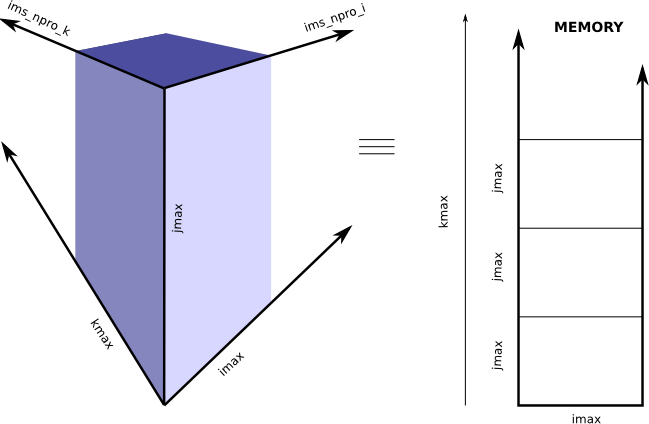
\includegraphics[height=0.8\textwidth,angle=270]{figs/parallel01a}
\caption{Domain decomposition of the global array of size {\tt
    imax\_total}$\times${\tt jmax\_total}$\times${\tt kmax\_total} into the the
  local arrays of size {\tt imax}$\times${\tt jmax}$\times${\tt kmax} using {\tt
  ims\_npro\_i} MPI tasks along the first (inner-most) index and {\tt
  ims\_npro\_k} along the last (outer-most) index. The structure in memory is
  shown in a two-dimensional array where the inner-most index runs up to {\tt
  imax} and the outer-most index runs up to {\tt jmax}$\times${\tt kmax}; it can
  also be interpreted as {\tt kmax} pages of size {\tt imax}$\times${\tt jmax}.}
\label{fig:parallel01a}
\end{centering}
\end{figure}

Two main transpositions are needed to perform the derivatives or any other
implicit operation in which we only need a set of complete lines along the
desired direction contiguously in memory. This is represented in
figure~\ref{fig:parallel01b}. For instance, if we need a derivative along $Ox$
of the field in array $a$, we can interpret the algorithm as follows. Consider
that array as {\tt jmax}$\times${\tt kmax} lines of size {\tt imax}, as
illustrated before in figure~\ref{fig:parallel01a}. Divide {\tt
jmax}$\times${\tt kmax}, the outer index, by {\tt ims\_npro\_i}, so as to have
precisely {\tt ims\_npro\_i} blocks (or colors) of size {\tt imax} times
whatever number you got before. Each of those blocks is send to the
corresponding processor. This operation is masked by creating an appropriate MPI
type, which is done during the initialization of the MPI part of the code. The
constraint we impose is that the ratio {\tt jmax}$\times${\tt kmax}/{\tt
ims\_npro\_i} needs to be an integer -- take this into account when defining the
grid. (This constraint could be avoided using padding, but we do not do it in
these main transposition operations.)

Let us consider now an implicit operation along $Oz$. For this case, each of the
pages {\tt imax}$\times${\tt jmax} needs to be divided by the number of tasks
{\tt ims\_npro\_k}, and this ratio is what needs to be an integer. It is also
seen in figure~\ref{fig:parallel01b} that now we need a stride in the MPI
type. The rest of the transposition algorithm is similar to the previous
case. The code variables containing the corresponding MPI types for the
transposition operations described in the previous and this paragraphs are {\tt
DNS\_MPI\_I\_PARTIAL} and {\tt DNS\_MPI\_K\_PARTIAL}, respectively.

\begin{figure}[!ht]
\begin{centering}
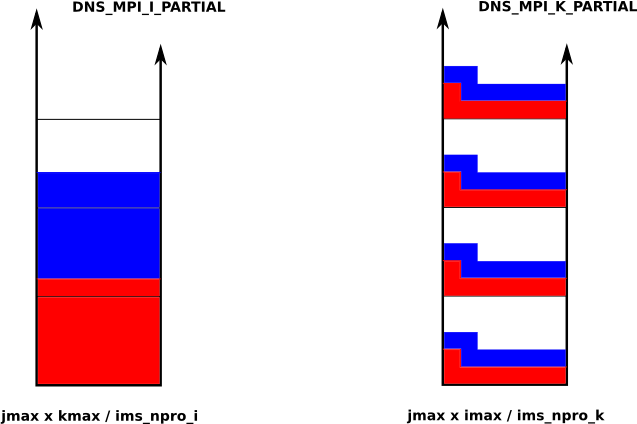
\includegraphics[height=0.8\textwidth,angle=270]{figs/parallel01b}
\caption{Memory management in transposition operations, from sketch in
  figure~\ref{fig:parallel01a}. Each color indicates the block of memory that
  goes into a common task. Based on these graphs, the offsets, strides and sizes
  in the MPI derived types are defined. The ratios at the bottom need to be an
  integer. You have as many colors as tasks involved in the corresponding
  transposition.}
\label{fig:parallel01b}
\end{centering}
\end{figure}

The I/O is done using MPI\_IO library. We read 
\begin{equation*}
{\tt ims\_npro}={\tt ims\_npro\_i} \times {\tt ims\_npro\_k} 
\end{equation*}
contiguous blocks of contiguous data, each block into one task. The
corresponding state is precisely equal to that obtained after the PARTIAL\_I
transposition, and so the only additional thing we need to do is an inverse
transposition of that type, and we already have the structure described in
figure~\ref{fig:parallel01a}. By this procedure we also defined the mapping,
which is sketched in figure~\ref{fig:parallel02}. From that mapping we see that
a task {\tt ims\_pro} contains the block given by
\begin{eqnarray*}
&{\tt ims\_pro\_i} = {\tt MOD(ims\_pro,ims\_npro\_i)}\\
&{\tt ims\_pro\_k} = {\tt INT(ims\_pro,ims\_npro\_i)}
\end{eqnarray*}

\begin{figure}[!ht]
\begin{centering}
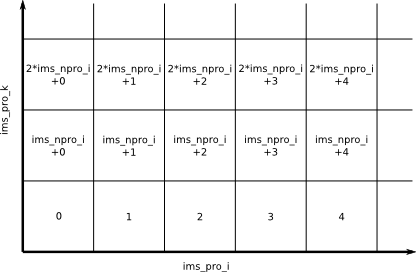
\includegraphics[height=0.6\textwidth,angle=270]{figs/parallel02}
\caption{Mapping.}
\label{fig:parallel02}
\end{centering}
\end{figure}

When needed, the information defining the boundary conditions is read from disk
using a similar procedure. we just need to define new MPI types for the
transposition along $Ox$ according to the specific size of the corresponding
arrays. This is done inside the I/O routines, as appropriate.

For the transpositions required in the Poisson equation, the procedure is
similar to the main algorithms defined above and shown in
figures~\ref{fig:parallel01a} and \ref{fig:parallel01b}, although two additional
planes in $Oy$ containing the boundary conditions, one at the bottom and one at
the top, and one in $Ox$ for the pseudo-Nyquist frequency are added (pseudo
meaning that only one should be added, but space is reserved in each processor
along that direction to keep the algorithm homogeneous; this could be
redefined). For these cases, padding is used inside each pages (defined above)
so that the only constraints in the grid are those imposed before in the two
major kinds of transposition. Hence, for a transposition along $Oz$, the same
structure as shown in figure~\ref{fig:parallel01b} is used but with a page of
size {\tt isize\_txc\_dimz} instead of {\tt imax}$\times${\tt jmax}, such that
{\tt isize\_txc\_dimz} is a multiple of 2$\times${\tt ims\_npro\_k}, (the factor
of 2 for real and imaginary parts of the same complex number to remain in the
same processor) and larger than ({\tt imax+2})$\times$({\tt jmax+2}). 

The same description applies to the transposition along $Ox$. The only
difference here is that a second type is added for the transformation without
the Nyquist frequency. This is used for instance for the first forward
transposition of data. {\em More here?}
